%%%%%%%%%%%%%%%%%%%%%%%%%%%%%%%%%%%%%%%%%%%%%%%%%%%%%%%%%%%%%%%%%%%%
\section{Organization}
\label{sec:fdsp-pd-org}
%\metainfo{\color{red}\bf  Content: Segreto/Warner}

The single-phase photon detector consortium has and will continue to benefit from the contributions of many institutions and facilities in Eruope and North and South America.  To help guide the interactions of these many contributors, the consortium is divided into six working groups, each with two or three conveners, to direct it's activities.   The structure of the organization is detailed below.

%%%%%%%%%%%%%%%%%%%%%%%%%%%%%%%%%%%
\subsection{Consortium Organization}
\label{sec:fdsp-pd-org-consortium}

The \single \dword{pds} consortium follows the typical organizational structure of DUNE consortia:
\begin{itemize}
\item A consortium lead
provides overall leadership for the effort, and attends meetings of the DUNE Executive and Technical Boards.
\item A technical lead 
provides technical support to the consortium lead, attends the Technical Board and other project meetings, oversees the project schedule and \dword{wbs}, and oversees the operation of the project working groups.  
%In the case of the \dword{pds}, the technical lead is supported by a deputy technical lead.
\end{itemize}

\begin{dunefigure}[PDS consortium organization chart]{fig:pds-org-chart}
{\dword{pds} consortium organization chart.}

	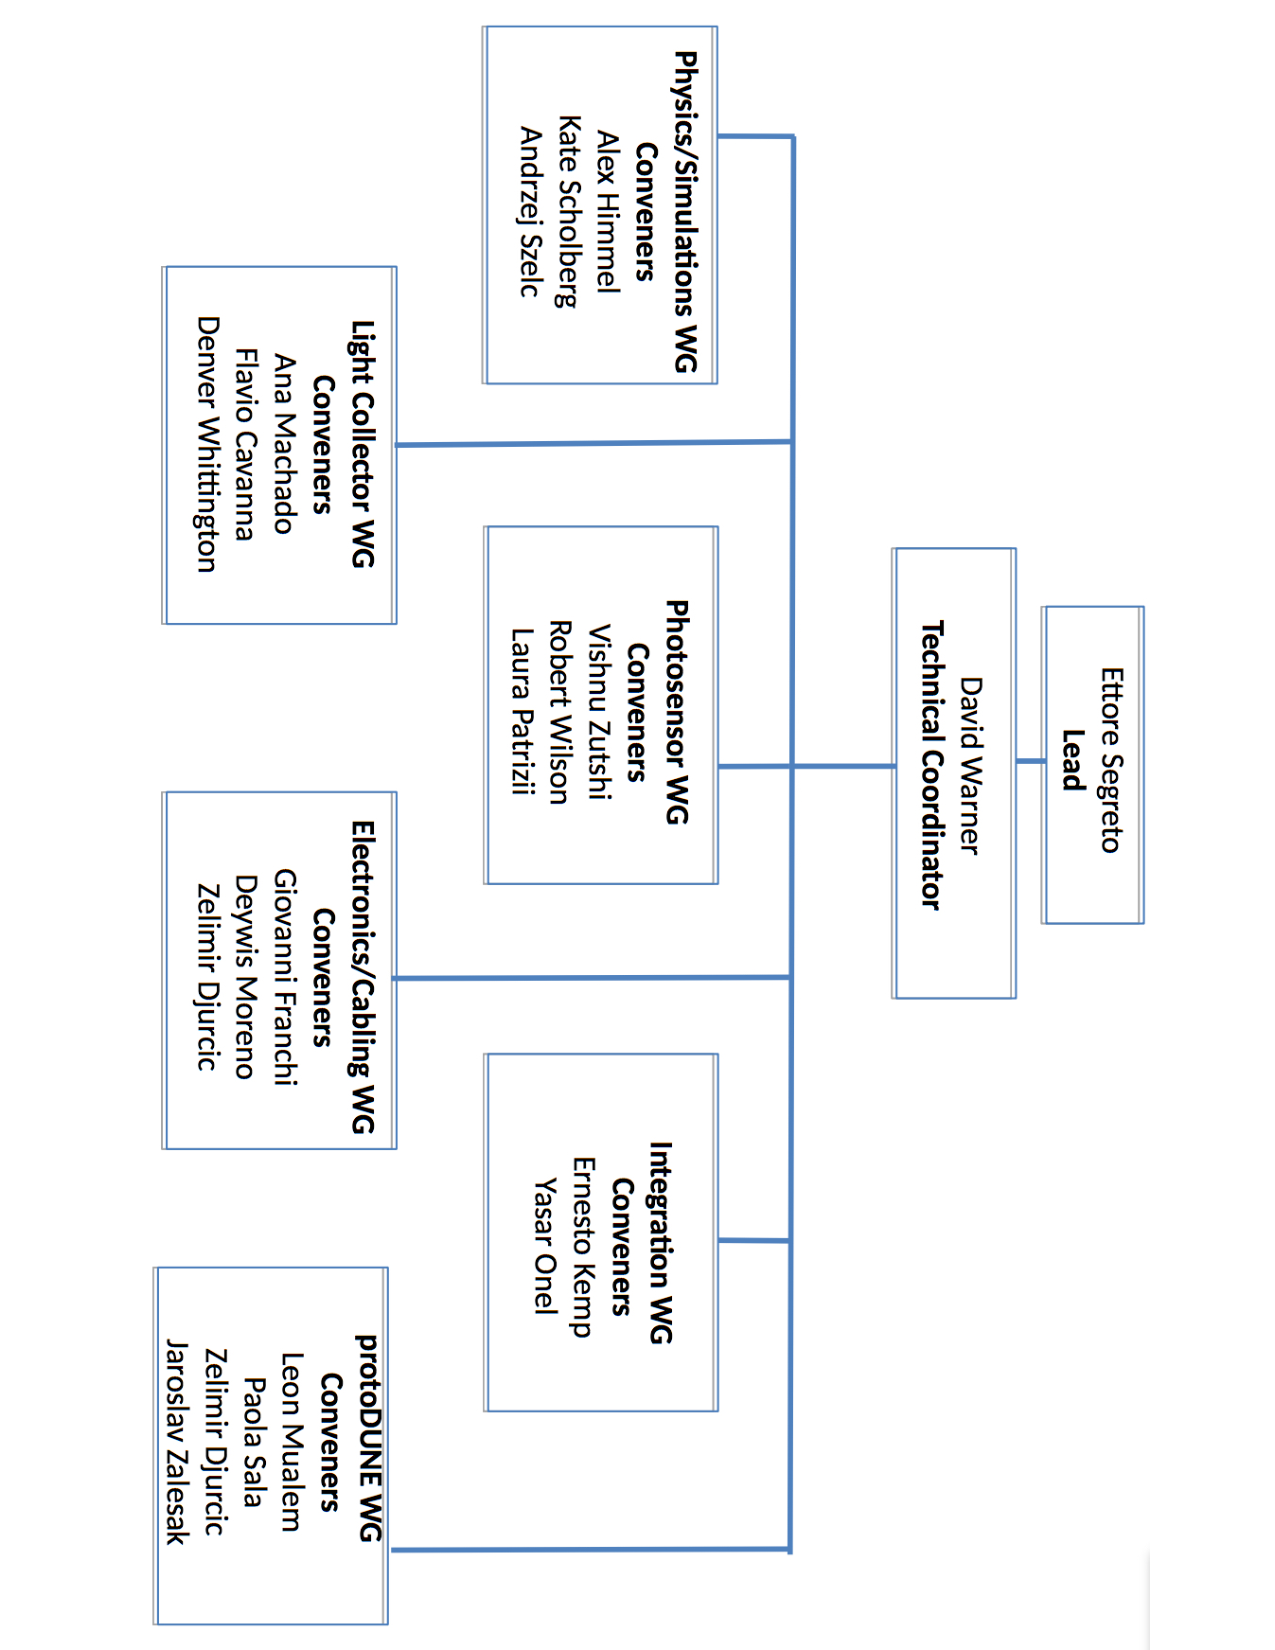
\includegraphics[angle=90,height=12cm]{pds-consortium-org-chart}
	
\end{dunefigure} 



Below the leadership, the consortium is divided up into six working groups, each led by two or three working group conveners as shown in Figure~\ref{fig:pds-org-chart}. 

%\fixme{Note that we have added the P-DUNE analysis working group}

% the \dword{pds} Management Table of Organization.  
Each working group is charged with one primary area of responsibility within the consortium, and the conveners report directly to the technical lead regarding those responsibilities.  As the consortium advances to a more detailed \dword{wbs} and project schedule, it is envisioned that each working group will be responsible for one section of those documents.

The working group conveners are appointed by the \dword{pds} project lead and technical lead, and the structure may evolve as the consortium matures and additional needs are identified. 

%%%%%%%%%%%%%%%%%%%%%%%%%%%%%%%%%%
\subsection{Planning Assumptions}
\label{sec:fdsp-pd-org-assmp}
%\metainfo{\color{blue} Content: Segreto/Warner}

Plans for the \dword{pds} consortium are based on the overall schedule for the DUNE \dword{fd}. In particular, the \dword{apa} schedule defines the time window for the completion of the final development program for the light collectors: A final down-select to a baseline light collector option and \dword{fe} electronics has been made for the TDR.  Due to the opportunities opened up by our new Italian colleaguesand their close connection with FBK, we may maintain an alternate photosensor option up to the pre-production review in September of 2020, but all other systems must be defined prior to the \dword{tdr}.

For planning purposes, we assume that the \dword{pds} modules will undergo final assembly and testing at one or more \dword{pds} assembly facilities, with an initial  assembly rate of approximately twenty modules per week, accelerating to forty modules per week in the second half of module fabrication.  These facilities are planned to be located in Latin America, primarily Brazil.

We further assume that the modules will be shipped from the fabrication facilities to the \dword{itf}, 
to be integrated along with the \dword{ce} into the \dword{apa} frames and cold tested in a cryogenic test facility.  We plan for an initial rate of two \dwords{apa} per week, with the possibility of accelerating to four \dwords{apa} per week as production lessons are learned.  \Dword{pds} personnel will be present at the integration facility to oversee the installation and testing.

%Meeting this timeline requires that the development of the ARAPUCA system be aggressively pursued throughout 2018, with a goal of testing near-final prototypes in the late fall of 2018 and allowing technology comparisons between the ARAPUCA and the light guide technologies in winter of 2019.

Additional development efforts will focus on:

\begin{itemize}
\item Identifying and selecting reliable cryogenic photosensor (\dword{sipm}) candidates,
\item Reducing cost and optimizing performance of \dword{fe} electronics,
\item Solidifying \dword{pds} performance requirements from additional physics simulation efforts.
\end{itemize}

We assume that apart from these items, where rapid development is still required, most of the detector components to be delivered by the \dword{pd} consortium will require only minor changes relative to the \dword{pdsp} components. For this reason, modifications of these other detector components will be delayed until 2019, which will also help with the funding profile. Exceptions will be made for further development in test stands with regard to cabling studies, and for the interface engineering required to ensure satisfactory integration of the \dword{pd} with the \dword{apa} and \dword{ce}  systems.

%%%%%%%%%%%%%%%%%%%%%%%%%%%%%%%%%%%
%\subsection{WBS and Responsibilities}
%\label{sec:fdsp-pd-org-wbs}
%\metainfo{\color{blue} Content: Warner/Mualem}

%%%%%%%%%%%%%%%%%%%%%%%%%%%%%%%%%%
\subsection{High-Level Schedule}
\label{sec:fdsp-pd-org-cs}
%\metainfo{\color{blue} Content: Warner/Mualem}

%The high-level schedule for the photon detector consortium through submission of the \dword{tdr} at the end of Q2 in FY19 is detailed in Figure~\ref{fig:pds-sched-to-tdr} and the pre-\dword{tdr} key milestones are listed in Table~\ref{fig:pds-pretdrkeymilestones}.

%\begin{dunefigure}[\dword{pd}S consortium schedule through to the \dword{tdr}.]{fig:pds-sched-to-tdr}
%{Photon Detector System consortium schedule through to the \dword{tdr}.}
 %%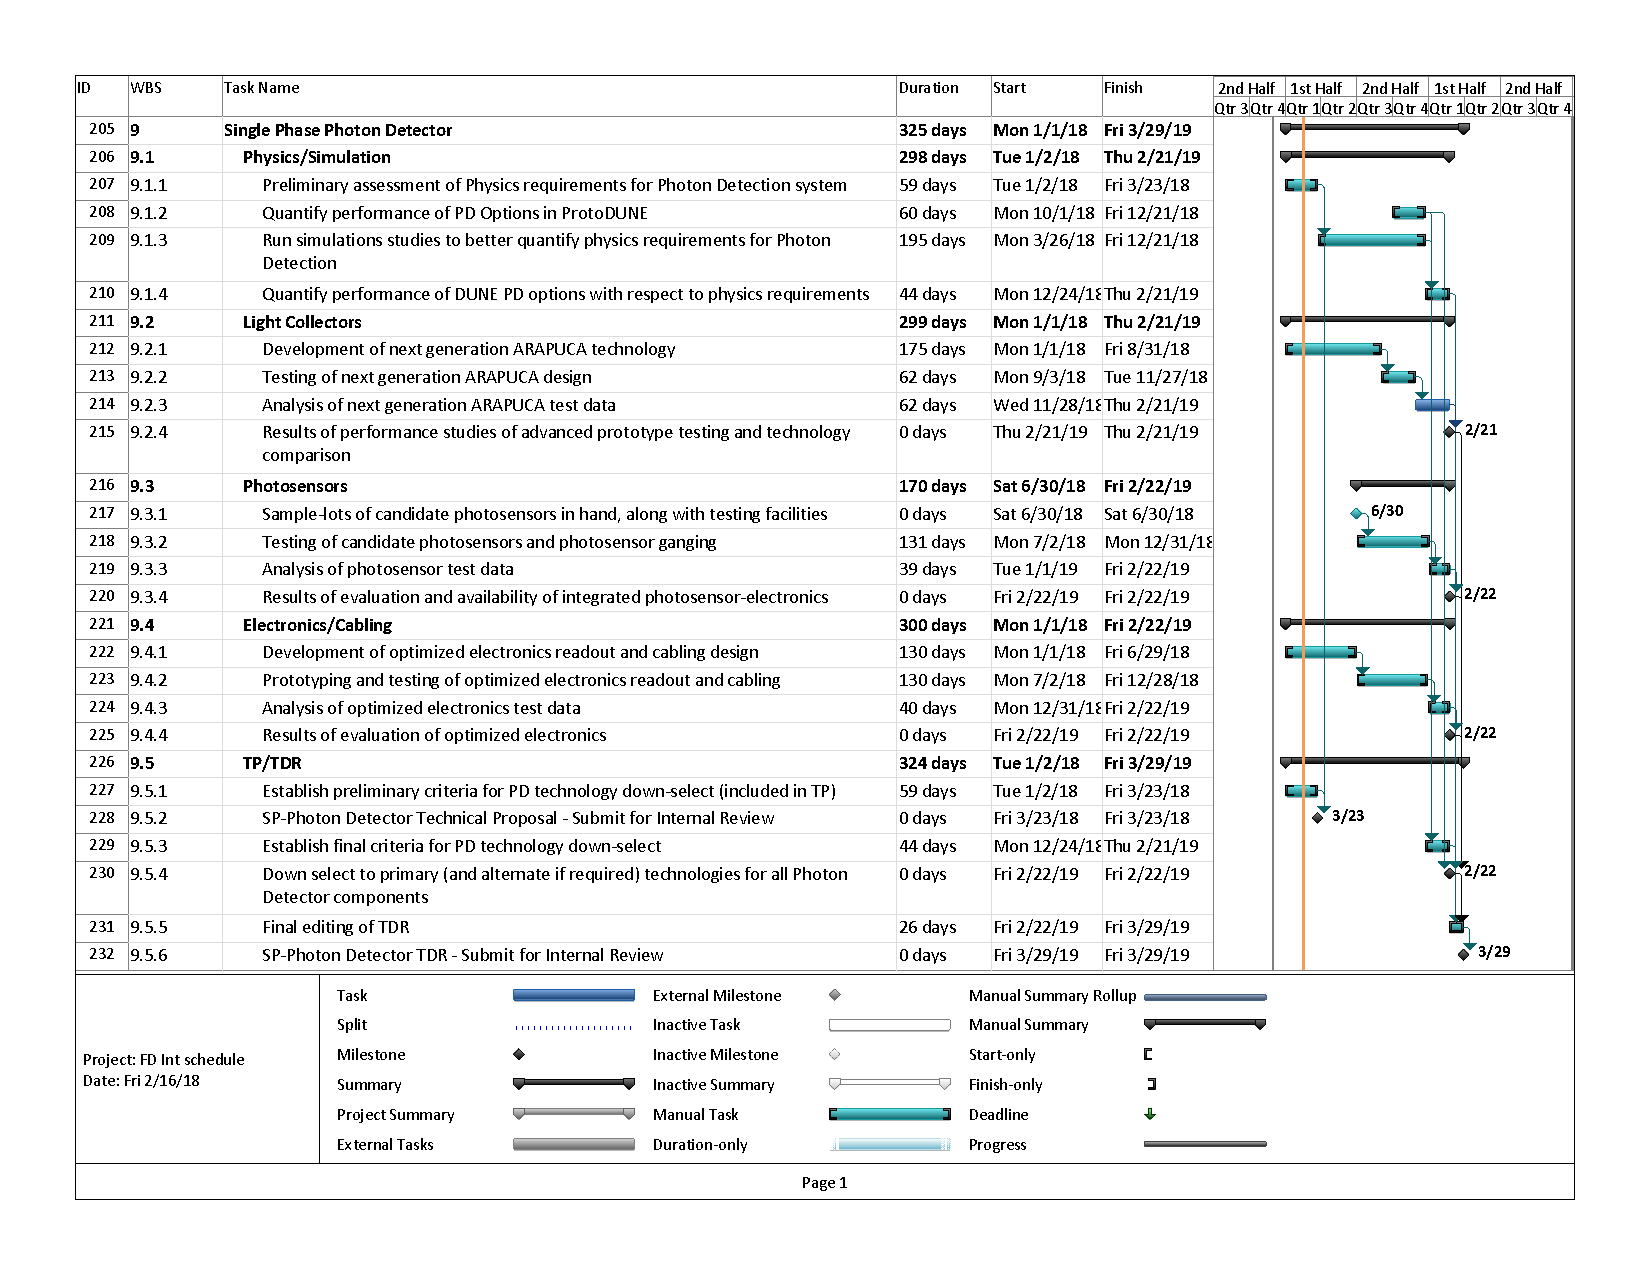
\includegraphics[width=1.0\columnwidth]{pds-sched-to-tdr.pdf}
%\end{dunefigure}

\fixme{Dave W:  this schedule will require updating I am discussing with Eric when ew might have a revised schedule.  Probably NOT by draft 2 in January}


\begin{dunetable}[Pre-\dword{tdr} key milestones.]
{ll}
{fig:pds-pretdrkeymilestones}
{Pre-\dword{tdr} key milestones.}
Milestone													&	Date	       \\ \toprowrule
Preliminary \dword{pd} technology selection criteria determined				&	03/21/18	\\ \colhline
Results from final prototype light collector studies available			&	02/21/19	\\ \colhline
Final \dword{pd} technology selection criteria available						&	02/21/19	\\ \colhline
Down-select to primary (and potential alternate) light collector technology	&	02/22/19	\\ \colhline
Submit initial \dword{tdr} draft for internal review							&	03/29/19	\\ 
\end{dunetable}

High-level post-\dword{tdr} milestones are listed in Table~\ref{fig:pds-posttdrkeymilestones}.

%LMM fixed detector -> Module below and 10 kt -> \SI{10}{kt}

\begin{dunetable}[Post-\dword{tdr} key milestones.]
{ll}
{fig:pds-posttdrkeymilestones}
{Post-\dword{tdr} key milestones.}
Milestone											&	Date	       \\ \toprowrule
\dword{pd} pre-production review(s) complete					&	03/2020 	\\ \colhline
Initial \dword{pd} module fabrication begins						&	09/2020	\\ \colhline
Final \dword{pd} production review based on initial production \dword{qa}		&	02/2021	\\ \colhline
First  \dword{pd} modules delivered for installation				&	05/2021	\\ \colhline
Installation into \dwords{apa} begins							&	06/2021     \\ \colhline
\dword{pd} fabrication complete (first \dword{spmod})			&	07/2023	\\ 
\end{dunetable}
